\documentclass[10pt]{article}
\usepackage[T1]{fontenc}
\usepackage{lmodern,amsmath,amssymb,graphicx,hyperref}
\usepackage[margin=0.8in]{geometry}
\setlength{\parindent}{0pt}
\setlength{\parskip}{6pt}
\begin{document}
\begin{center}
{\Large Exact weighted monomial counts}\\[4pt]
Prime norm study, 14 November 2026\\
Source freeze \texttt{740732e95389e5185ed9a6547c18d8d889a6c580}
\end{center}

\textbf{Result.} For positive natural weights $w_1,\ldots,w_v$, let
$M(w,D)$ count \emph{every} exponent vector $e\in\mathbb N^v$ with
$\sum_i w_i e_i\le D$. The new Lean module establishes
\[
 M(w,D)\prod_i w_i\ \le\ \binom{D+\sum_i w_i}{v},\qquad
 M(w,D)\prod_i w_i\,v!\ \le\ (D+\sum_i w_i)^v.
\]
For consecutive weights this gives
\[
 \boxed{M(v,D)(v!)^2\le(D+v^2)^v.}
\]
PCC-20261114-cc1d70 / 621b19 / 9932d5; unsigned [pcc:unverified].
The exact binomial inequality is retained, rather than only the coarser
square bound. Zero variables and zero budget are included.

\textbf{Proof mechanism.} Attach digits $0\le t_i<w_i$ and set
$y_i=w_i e_i+t_i$. Euclidean division recovers both $e_i$ and $t_i$,
so the map is injective. Also
$\sum_i y_i\le L:=D+\sum_i(w_i-1)$.
Encode $y$ as a multiset with $y_i$ copies of label $i$ and
$L-\sum_i y_i$ copies of an extra slack label. Its cardinality is $L$;
counts of the ordinary labels recover $y$. Mathlib stars-and-bars counts
these multisets by $\binom{L+v}{v}$. Positive weights give
$L+v=D+\sum_i w_i$. The descending-factorial bound supplies the second
inequality. For weights $1,\ldots,v$, the product is $v!$ and
$\sum_i w_i\le v^2$.

\textbf{Completeness of the counted set.} The executable finite set is a
box $0\le e_i\le D$ filtered by weighted degree. The theorem
\texttt{mem\_monomials} proves equivalence to the weighted inequality for
positive weights. No support list or moment oracle is supplied.

\textbf{Application boundary.} This is finite combinatorics, with no
claim of novelty for the elementary argument. It does not prove that the
growing norm inputs have this grading or that their full iterated closure
stabilizes at a small cutoff. Public base coverage, signed output,
extraction, failed attempts and complete expected bit cost remain explicit
application obligations. An original $W_{\rm new}=W_{\rm base}+CH$ jet
map is not established by the counting theorem.

\newpage
\begin{center}
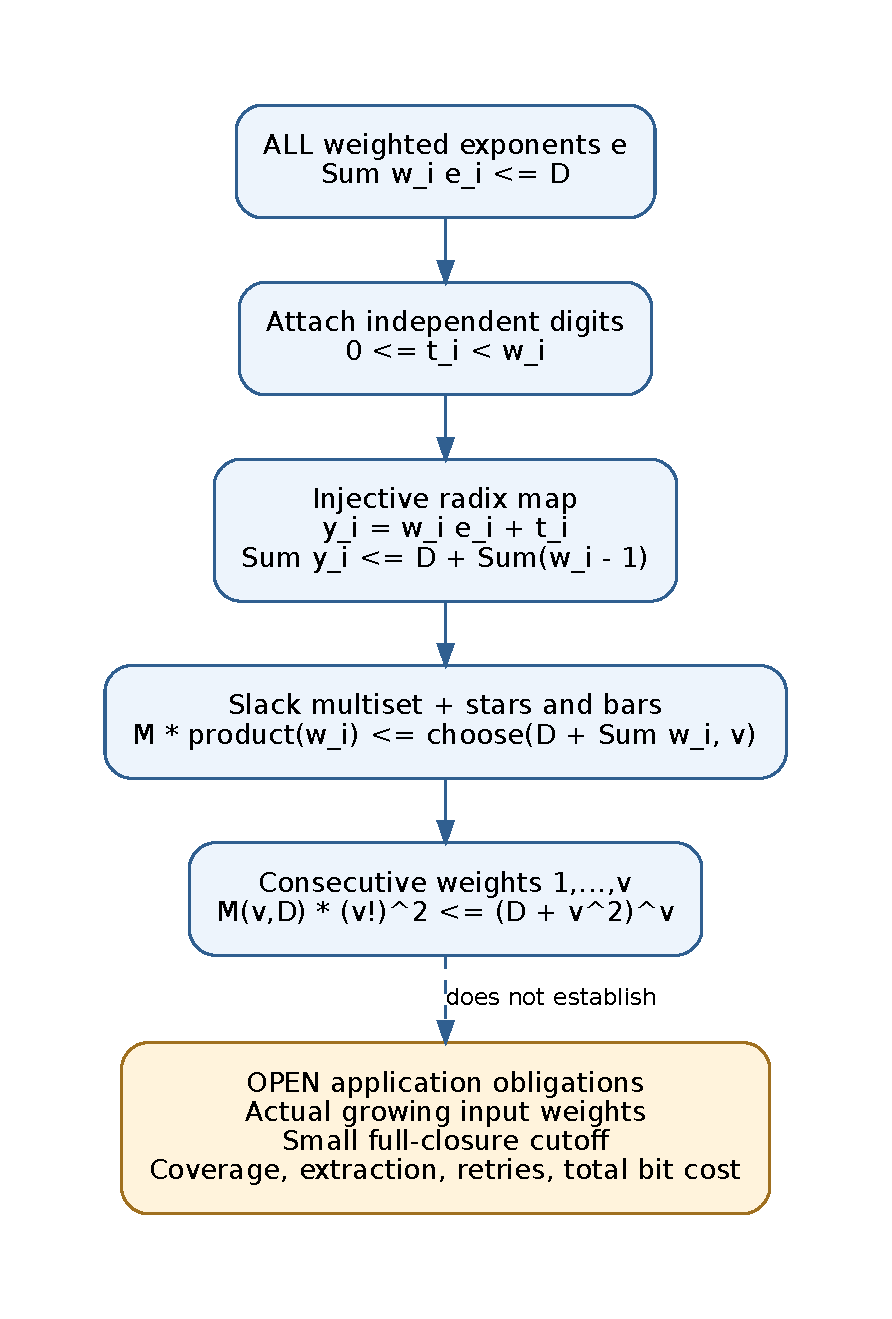
\includegraphics[height=0.64\textheight]{count.pdf}
\end{center}
\textbf{Evidence and sources.} Source:
\texttt{lean/NormWeightedCount.lean}, ten authored theorems;
exact declaration hashes in \texttt{weighted-count-evidence/claim-pins.json}.
Build drafts 001 and 002 failed on elaboration/API usage and remain
archived with their source; build003 exits0 without warnings.
Gate and fresh replay receipts are recorded in the companion README.
Unsigned claims do not assert signed standing.

Pinned Mathlib sources:\\
\path{Data/Sym/Card.lean}\\
\path{Data/Nat/Choose/Bounds.lean}\\
\path{Data/Nat/Factorial/BigOperators.lean}.


Prior-work review read actual P1514 producer/audit and P1536 norm-jet audit
at crypto-autoresearcher \texttt{14f7a739d}. P1514's dense cutoff was
sufficient, not a universal minimum. P1536's exact norm-jet inverse lacked
a cheap constructor. Neither audit is an experiment measuring early
weighted closure. KB tools and wrapper executable were unavailable.

No native fixture, solver, timing campaign, paid job or Python cryptomath
was run. No canonical performance graph changes: no measured performance
result is added.
\end{document}
